\documentclass[11pt,letterpaper]{article}
\usepackage[lmargin=1in,rmargin=1in,tmargin=1in,bmargin=1in]{geometry}

% -------------------
% Packages
% -------------------
\usepackage{
	amsmath,			% Math Environments
	amssymb,			% Extended Symbols
	enumerate,		% Enumerate Environments
	graphicx,			% Include Images    
	lastpage,			% Reference Lastpage
	multicol,			% Use Multi-columns
	multirow,			% Use Multi-rows
	siunitx
}

\graphicspath{{./images/}}

\usepackage{wrapfig}

% -------------------
% Font
% -------------------
\usepackage[T1]{fontenc}
\usepackage{charter}    


% -------------------
% Heading Commands
% -------------------
\newcommand{\class}{Mu Alpha Theta}
\newcommand{\term}{2022-2023}
\newcommand{\head}[2]{%
\thispagestyle{empty}
\vspace*{-0.5in}
\noindent\begin{tabular*}{\textwidth}{l @{\extracolsep{\fill}} r @{\extracolsep{6pt}} l}
	\textbf{#1} & \textbf{Name:} & \makebox[5.75cm]{\hrulefill} \\
	\textbf{#2} & & \\
	\textbf{\class:\; \term} & & \\
\end{tabular*} \\
\rule[2ex]{\textwidth}{2pt} %
}


% -------------------
% Commands
% -------------------
\newcommand{\prob}{\noindent\textbf{Problem. }}
\newcounter{problem}
\newcommand{\problem}{
	\stepcounter{problem}%
	\noindent \textbf{Problem \theproblem. }%
}
\newcommand{\pointproblem}[1]{
	\stepcounter{problem}%
	\noindent \textbf{Problem \theproblem.} (#1 points)\,%
}
\newcommand{\pspace}{\par\vspace{\baselineskip}}
\newcommand{\ds}{\displaystyle}


% -------------------
% Header & Footer
% -------------------
\usepackage{fancyhdr}

\fancypagestyle{pages}{
	%Headers
	\fancyhead[L]{}
	\fancyhead[C]{}
	\fancyhead[R]{}
\renewcommand{\headrulewidth}{0pt}
	%Footers
	\fancyfoot[L]{}
	\fancyfoot[C]{}
	\fancyfoot[R]{}
\renewcommand{\footrulewidth}{0.0pt}
}
\headheight=0pt
\footskip=14pt

\pagestyle{pages}


% -------------------
% Content
% -------------------

\begin{document}
\head{Worksheet \#2}{Date:}
\centering

% Question 1: https://artofproblemsolving.com/wiki/index.php/2010_AMC_8_Problems/Problem_23
\begin{minipage}{\textwidth}
     \problem

     \begin{wrapfigure}[11]{r}{0.6\textwidth}
          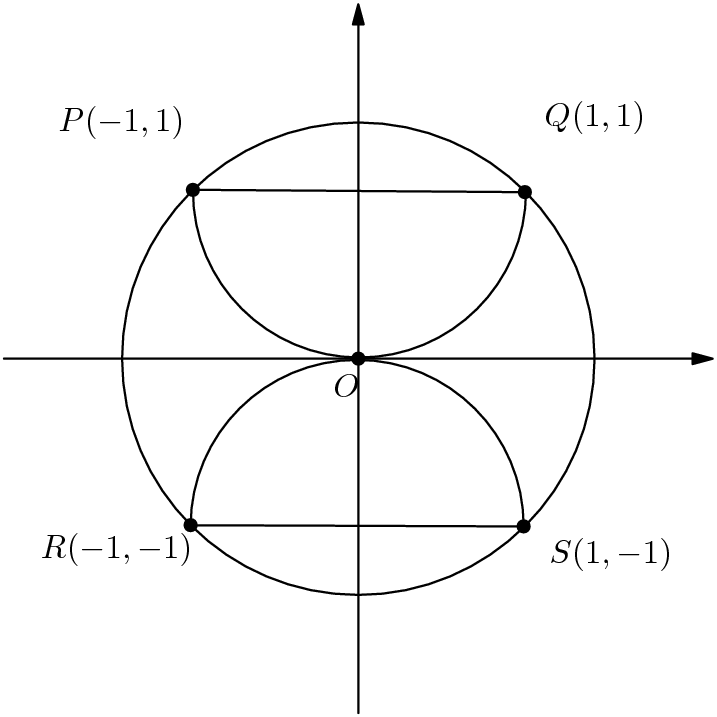
\includegraphics[height = 8cm]{images/AMC-8-2010-P23.png}
     \end{wrapfigure}
     \noindent Semicircles $POQ$ and $ROS$ pass through the center $O$. What is the ratio of the combined areas of the two semicircles to the circle? \vspace{2cm}
\end{minipage}
\vspace{8cm}

% Question 2: https://artofproblemsolving.com/wiki/index.php/2009_AMC_12A_Problems/Problem_11
\begin{minipage}{\textwidth}
     \problem

     
     \noindent The figures $F_1$, $F_2$, $F_3$, and $F_4$ shown are the first in a sequence of figures. For $n\ge3$, $F_n$ is constructed from $F_{n - 1}$ by surrounding it with a square and placing one more diamond on each side of the new square than $F_{n - 1}$ had on each side of its outside square. For example, figure $F_3$ has $13$ diamonds. How many diamonds are there in figure $F_{20}$?

     \vspace{1cm}

     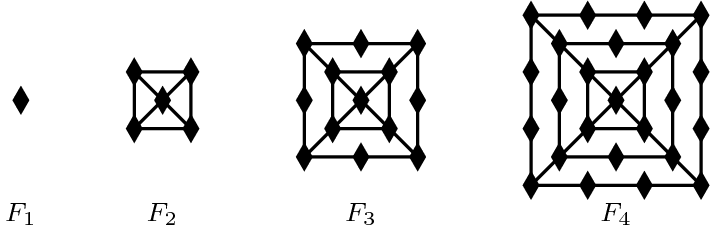
\includegraphics[width = 8cm]{images/AMC-12-2009-P11.png}   

\end{minipage}
\vspace{2cm}

% Question 3: https://artofproblemsolving.com/wiki/index.php/2006_AMC_10A_Problems/Problem_12
\begin{minipage}{\textwidth}
     \problem

     \noindent Rolly wishes to secure his dog with an 8-foot rope to a square shed that is 16 feet on each side. His preliminary drawings are shown. Assume that the area around the shed is unbounded with no obstacles. Which arrangment gives the greatest area to roam, and by how many square feet? Give an answer in exact form.
     
     \vspace{1cm}

     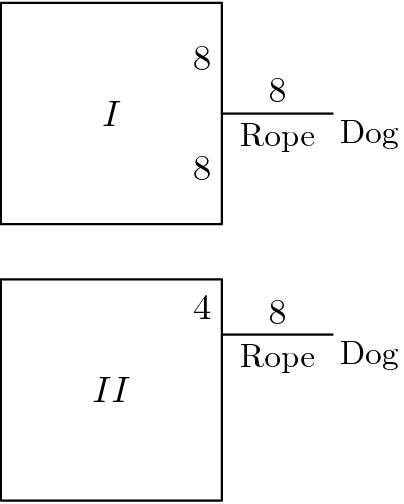
\includegraphics[height = 4cm]{images/AMC-10-2006-P12.png}
     
\end{minipage}
\vspace{2cm}

% Question 4: https://artofproblemsolving.com/wiki/index.php/2007_AMC_10A_Problems/Problem_15
\begin{minipage}{\textwidth}
     \problem

     \noindent Four circles of radius $1$ are each tangent to two sides of a square and externally tangent to a circle of radius $2$, as shown. What is the area of the square?

     \vspace{1cm}
     
     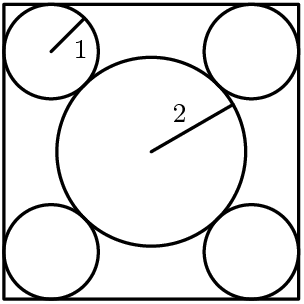
\includegraphics[width=0.25\textwidth]{images/AMC-10-2007-P15.png}

\end{minipage}
\vspace{2cm}

% Question 5: https://artofproblemsolving.com/wiki/index.php/2016_AMC_10B_Problems/Problem_19
\begin{minipage}{\textwidth}
     \problem
     
     \begin{wrapfigure}[11]{r}{0.35\textwidth}
          \hspace{1.5cm}
          \vspace{-0.5cm}
          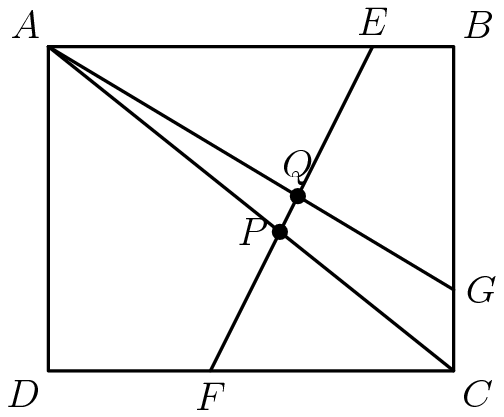
\includegraphics[width = 5cm]{images/AMC-10-2016-P19.png}
     \end{wrapfigure}

     \noindent Rectangle $ABCD$ has $AB=5$ and $BC=4$. Point $E$ lies on $\overline{AB}$ so that $EB=1$, point $G$ lies on $\overline{BC}$ so that $CG=1$. and point $F$ lies on $\overline{CD}$ so that $DF=2$. Segments $\overline{AG}$ and $\overline{AC}$ intersect $\overline{EF}$ at $Q$ and $P$, respectively. What is the value of $\frac{PQ}{EF}$?

\end{minipage}


\vspace{2cm}

\end{document}